\documentclass[twoside]{book}

% Packages required by doxygen
\usepackage{fixltx2e}
\usepackage{calc}
\usepackage{doxygen}
\usepackage[export]{adjustbox} % also loads graphicx
\usepackage{graphicx}
\usepackage[utf8]{inputenc}
\usepackage{makeidx}
\usepackage{multicol}
\usepackage{multirow}
\PassOptionsToPackage{warn}{textcomp}
\usepackage{textcomp}
\usepackage[nointegrals]{wasysym}
\usepackage[table]{xcolor}

% Font selection
\usepackage[T1]{fontenc}
\usepackage[scaled=.90]{helvet}
\usepackage{courier}
\usepackage{amssymb}
\usepackage{sectsty}
\renewcommand{\familydefault}{\sfdefault}
\allsectionsfont{%
  \fontseries{bc}\selectfont%
  \color{darkgray}%
}
\renewcommand{\DoxyLabelFont}{%
  \fontseries{bc}\selectfont%
  \color{darkgray}%
}
\newcommand{\+}{\discretionary{\mbox{\scriptsize$\hookleftarrow$}}{}{}}

% Page & text layout
\usepackage{geometry}
\geometry{%
  a4paper,%
  top=2.5cm,%
  bottom=2.5cm,%
  left=2.5cm,%
  right=2.5cm%
}
\tolerance=750
\hfuzz=15pt
\hbadness=750
\setlength{\emergencystretch}{15pt}
\setlength{\parindent}{0cm}
\setlength{\parskip}{3ex plus 2ex minus 2ex}
\makeatletter
\renewcommand{\paragraph}{%
  \@startsection{paragraph}{4}{0ex}{-1.0ex}{1.0ex}{%
    \normalfont\normalsize\bfseries\SS@parafont%
  }%
}
\renewcommand{\subparagraph}{%
  \@startsection{subparagraph}{5}{0ex}{-1.0ex}{1.0ex}{%
    \normalfont\normalsize\bfseries\SS@subparafont%
  }%
}
\makeatother

% Headers & footers
\usepackage{fancyhdr}
\pagestyle{fancyplain}
\fancyhead[LE]{\fancyplain{}{\bfseries\thepage}}
\fancyhead[CE]{\fancyplain{}{}}
\fancyhead[RE]{\fancyplain{}{\bfseries\leftmark}}
\fancyhead[LO]{\fancyplain{}{\bfseries\rightmark}}
\fancyhead[CO]{\fancyplain{}{}}
\fancyhead[RO]{\fancyplain{}{\bfseries\thepage}}
\fancyfoot[LE]{\fancyplain{}{}}
\fancyfoot[CE]{\fancyplain{}{}}
\fancyfoot[RE]{\fancyplain{}{\bfseries\scriptsize Generated by Doxygen }}
\fancyfoot[LO]{\fancyplain{}{\bfseries\scriptsize Generated by Doxygen }}
\fancyfoot[CO]{\fancyplain{}{}}
\fancyfoot[RO]{\fancyplain{}{}}
\renewcommand{\footrulewidth}{0.4pt}
\renewcommand{\chaptermark}[1]{%
  \markboth{#1}{}%
}
\renewcommand{\sectionmark}[1]{%
  \markright{\thesection\ #1}%
}

% Indices & bibliography
\usepackage{natbib}
\usepackage[titles]{tocloft}
\setcounter{tocdepth}{3}
\setcounter{secnumdepth}{5}
\makeindex

% Hyperlinks (required, but should be loaded last)
\usepackage{ifpdf}
\ifpdf
  \usepackage[pdftex,pagebackref=true]{hyperref}
\else
  \usepackage[ps2pdf,pagebackref=true]{hyperref}
\fi
\hypersetup{%
  colorlinks=true,%
  linkcolor=blue,%
  citecolor=blue,%
  unicode%
}

% Custom commands
\newcommand{\clearemptydoublepage}{%
  \newpage{\pagestyle{empty}\cleardoublepage}%
}

\usepackage{caption}
\captionsetup{labelsep=space,justification=centering,font={bf},singlelinecheck=off,skip=4pt,position=top}

%===== C O N T E N T S =====

\begin{document}

% Titlepage & ToC
\hypersetup{pageanchor=false,
             bookmarksnumbered=true,
             pdfencoding=unicode
            }
\pagenumbering{alph}
\begin{titlepage}
\vspace*{7cm}
\begin{center}%
{\Large Digital Terrain Model project }\\
\vspace*{1cm}
{\large Generated by Doxygen 1.8.13}\\
\end{center}
\end{titlepage}
\clearemptydoublepage
\pagenumbering{roman}
\tableofcontents
\clearemptydoublepage
\pagenumbering{arabic}
\hypersetup{pageanchor=true}

%--- Begin generated contents ---
\chapter{Class Index}
\section{Class List}
Here are the classes, structs, unions and interfaces with brief descriptions\+:\begin{DoxyCompactList}
\item\contentsline{section}{\hyperlink{structdelaunator_1_1compare}{delaunator\+::compare} }{\pageref{structdelaunator_1_1compare}}{}
\item\contentsline{section}{\hyperlink{classdelaunator_1_1Delaunator}{delaunator\+::\+Delaunator} }{\pageref{classdelaunator_1_1Delaunator}}{}
\item\contentsline{section}{\hyperlink{structdelaunator_1_1DelaunatorPoint}{delaunator\+::\+Delaunator\+Point} }{\pageref{structdelaunator_1_1DelaunatorPoint}}{}
\item\contentsline{section}{\hyperlink{classImage}{Image} \\*A class defining a custom image with some classic attributes \+: }{\pageref{classImage}}{}
\item\contentsline{section}{\hyperlink{structMNT}{M\+NT} \\*Digital Terrain Model structure (D\+TM or \hyperlink{structMNT}{M\+NT} in French) composed of\+: }{\pageref{structMNT}}{}
\item\contentsline{section}{\hyperlink{classPixel}{Pixel} \\*A class defining a custom pixel \+: R\+GB components with custom attributes \+: }{\pageref{classPixel}}{}
\end{DoxyCompactList}

\chapter{File Index}
\section{File List}
Here is a list of all documented files with brief descriptions\+:\begin{DoxyCompactList}
\item\contentsline{section}{src/\hyperlink{delaunator_8hpp}{delaunator.\+hpp} }{\pageref{delaunator_8hpp}}{}
\item\contentsline{section}{src/\hyperlink{Image_8h}{Image.\+h} }{\pageref{Image_8h}}{}
\item\contentsline{section}{src/\hyperlink{Pixel_8h}{Pixel.\+h} }{\pageref{Pixel_8h}}{}
\item\contentsline{section}{src/\hyperlink{utils_8h}{utils.\+h} \\*A file containing useful structure and functions to generate a D\+TM or \hyperlink{structMNT}{M\+NT} in French }{\pageref{utils_8h}}{}
\end{DoxyCompactList}

\chapter{Class Documentation}
\hypertarget{structdelaunator_1_1compare}{}\section{delaunator\+:\+:compare Struct Reference}
\label{structdelaunator_1_1compare}\index{delaunator\+::compare@{delaunator\+::compare}}
\subsection*{Public Member Functions}
\begin{DoxyCompactItemize}
\item 
\mbox{\Hypertarget{structdelaunator_1_1compare_a78b94657ec7bad085353f318365fa20a}\label{structdelaunator_1_1compare_a78b94657ec7bad085353f318365fa20a}} 
bool {\bfseries operator()} (std\+::size\+\_\+t i, std\+::size\+\_\+t j)
\end{DoxyCompactItemize}
\subsection*{Public Attributes}
\begin{DoxyCompactItemize}
\item 
\mbox{\Hypertarget{structdelaunator_1_1compare_a28fe3e7cd51ef236ac051fb47421321a}\label{structdelaunator_1_1compare_a28fe3e7cd51ef236ac051fb47421321a}} 
std\+::vector$<$ double $>$ const  \& {\bfseries coords}
\item 
\mbox{\Hypertarget{structdelaunator_1_1compare_a71238f2868c76ee8048cdd72d58da65c}\label{structdelaunator_1_1compare_a71238f2868c76ee8048cdd72d58da65c}} 
double {\bfseries cx}
\item 
\mbox{\Hypertarget{structdelaunator_1_1compare_ad8f7ce42823fff74a6062e439f93682d}\label{structdelaunator_1_1compare_ad8f7ce42823fff74a6062e439f93682d}} 
double {\bfseries cy}
\end{DoxyCompactItemize}


The documentation for this struct was generated from the following file\+:\begin{DoxyCompactItemize}
\item 
src/\hyperlink{delaunator_8hpp}{delaunator.\+hpp}\end{DoxyCompactItemize}

\hypertarget{classdelaunator_1_1Delaunator}{}\section{delaunator\+:\+:Delaunator Class Reference}
\label{classdelaunator_1_1Delaunator}\index{delaunator\+::\+Delaunator@{delaunator\+::\+Delaunator}}
\subsection*{Public Member Functions}
\begin{DoxyCompactItemize}
\item 
\mbox{\Hypertarget{classdelaunator_1_1Delaunator_a094e288531f1695ca64437f0c04128c8}\label{classdelaunator_1_1Delaunator_a094e288531f1695ca64437f0c04128c8}} 
{\bfseries Delaunator} (std\+::vector$<$ double $>$ const \&in\+\_\+coords)
\item 
\mbox{\Hypertarget{classdelaunator_1_1Delaunator_ae6ee753d08679728afd4b603eab7d1ab}\label{classdelaunator_1_1Delaunator_ae6ee753d08679728afd4b603eab7d1ab}} 
double {\bfseries get\+\_\+hull\+\_\+area} ()
\end{DoxyCompactItemize}
\subsection*{Public Attributes}
\begin{DoxyCompactItemize}
\item 
\mbox{\Hypertarget{classdelaunator_1_1Delaunator_ac48ad29af151d66885120872bf46f750}\label{classdelaunator_1_1Delaunator_ac48ad29af151d66885120872bf46f750}} 
std\+::vector$<$ double $>$ const  \& {\bfseries coords}
\item 
\mbox{\Hypertarget{classdelaunator_1_1Delaunator_a6b613da33302f09aaea8fd74663d61cb}\label{classdelaunator_1_1Delaunator_a6b613da33302f09aaea8fd74663d61cb}} 
std\+::vector$<$ std\+::size\+\_\+t $>$ {\bfseries triangles}
\item 
\mbox{\Hypertarget{classdelaunator_1_1Delaunator_aff04629e1166358e4f2d43ed1e6524ef}\label{classdelaunator_1_1Delaunator_aff04629e1166358e4f2d43ed1e6524ef}} 
std\+::vector$<$ std\+::size\+\_\+t $>$ {\bfseries halfedges}
\item 
\mbox{\Hypertarget{classdelaunator_1_1Delaunator_a9d0f92cb1eee39f5ac80f65495d543c3}\label{classdelaunator_1_1Delaunator_a9d0f92cb1eee39f5ac80f65495d543c3}} 
std\+::vector$<$ std\+::size\+\_\+t $>$ {\bfseries hull\+\_\+prev}
\item 
\mbox{\Hypertarget{classdelaunator_1_1Delaunator_a8e6c50f7a0ff8c8b1f6e62c92004f57c}\label{classdelaunator_1_1Delaunator_a8e6c50f7a0ff8c8b1f6e62c92004f57c}} 
std\+::vector$<$ std\+::size\+\_\+t $>$ {\bfseries hull\+\_\+next}
\item 
\mbox{\Hypertarget{classdelaunator_1_1Delaunator_af9da27b2b5f8dc5b916b474078dd093a}\label{classdelaunator_1_1Delaunator_af9da27b2b5f8dc5b916b474078dd093a}} 
std\+::vector$<$ std\+::size\+\_\+t $>$ {\bfseries hull\+\_\+tri}
\item 
\mbox{\Hypertarget{classdelaunator_1_1Delaunator_a28717862d3ea8ae531ee2dc7fb57b639}\label{classdelaunator_1_1Delaunator_a28717862d3ea8ae531ee2dc7fb57b639}} 
std\+::size\+\_\+t {\bfseries hull\+\_\+start}
\end{DoxyCompactItemize}


The documentation for this class was generated from the following file\+:\begin{DoxyCompactItemize}
\item 
src/\hyperlink{delaunator_8hpp}{delaunator.\+hpp}\end{DoxyCompactItemize}

\hypertarget{structdelaunator_1_1DelaunatorPoint}{}\section{delaunator\+:\+:Delaunator\+Point Struct Reference}
\label{structdelaunator_1_1DelaunatorPoint}\index{delaunator\+::\+Delaunator\+Point@{delaunator\+::\+Delaunator\+Point}}
\subsection*{Public Attributes}
\begin{DoxyCompactItemize}
\item 
\mbox{\Hypertarget{structdelaunator_1_1DelaunatorPoint_aa86be67d87cfc564557b05786ee0213b}\label{structdelaunator_1_1DelaunatorPoint_aa86be67d87cfc564557b05786ee0213b}} 
std\+::size\+\_\+t {\bfseries i}
\item 
\mbox{\Hypertarget{structdelaunator_1_1DelaunatorPoint_a6d0cf1b98a5ec895fcac5c1c2a10b926}\label{structdelaunator_1_1DelaunatorPoint_a6d0cf1b98a5ec895fcac5c1c2a10b926}} 
double {\bfseries x}
\item 
\mbox{\Hypertarget{structdelaunator_1_1DelaunatorPoint_a9137c3a0356dfc8a330b34f2944864a5}\label{structdelaunator_1_1DelaunatorPoint_a9137c3a0356dfc8a330b34f2944864a5}} 
double {\bfseries y}
\item 
\mbox{\Hypertarget{structdelaunator_1_1DelaunatorPoint_ab35213b07c403aa7ff3d927c7ca0d464}\label{structdelaunator_1_1DelaunatorPoint_ab35213b07c403aa7ff3d927c7ca0d464}} 
std\+::size\+\_\+t {\bfseries t}
\item 
\mbox{\Hypertarget{structdelaunator_1_1DelaunatorPoint_ab72027bce56e71be2d68440fbf261722}\label{structdelaunator_1_1DelaunatorPoint_ab72027bce56e71be2d68440fbf261722}} 
std\+::size\+\_\+t {\bfseries prev}
\item 
\mbox{\Hypertarget{structdelaunator_1_1DelaunatorPoint_aa6196f04bd176a2648d63f9235212f6b}\label{structdelaunator_1_1DelaunatorPoint_aa6196f04bd176a2648d63f9235212f6b}} 
std\+::size\+\_\+t {\bfseries next}
\item 
\mbox{\Hypertarget{structdelaunator_1_1DelaunatorPoint_ad2b84b88913a220615d6179ea6283b0d}\label{structdelaunator_1_1DelaunatorPoint_ad2b84b88913a220615d6179ea6283b0d}} 
bool {\bfseries removed}
\end{DoxyCompactItemize}


The documentation for this struct was generated from the following file\+:\begin{DoxyCompactItemize}
\item 
src/\hyperlink{delaunator_8hpp}{delaunator.\+hpp}\end{DoxyCompactItemize}

\hypertarget{classImage}{}\section{Image Class Reference}
\label{classImage}\index{Image@{Image}}


A class defining a custom image with some classic attributes \+:  




{\ttfamily \#include $<$Image.\+h$>$}

\subsection*{Public Member Functions}
\begin{DoxyCompactItemize}
\item 
\mbox{\Hypertarget{classImage_a58edd1c45b4faeb5f789b0d036d02313}\label{classImage_a58edd1c45b4faeb5f789b0d036d02313}} 
\hyperlink{classImage_a58edd1c45b4faeb5f789b0d036d02313}{Image} ()
\begin{DoxyCompactList}\small\item\em Default constructor \+: construct a new \hyperlink{classImage}{Image} object. \end{DoxyCompactList}\item 
\hyperlink{classImage_a05264c84d006ceb2e4f4405561999c5f}{Image} (const int width, const float xmin, const float xmax, const float ymin, const float ymax, bool gray, bool binary)
\begin{DoxyCompactList}\small\item\em Construct a new \hyperlink{classImage}{Image} object. \end{DoxyCompactList}\item 
\mbox{\Hypertarget{classImage_aacd6d371d5f6d56a0c4070b0fbfb1f03}\label{classImage_aacd6d371d5f6d56a0c4070b0fbfb1f03}} 
void \hyperlink{classImage_aacd6d371d5f6d56a0c4070b0fbfb1f03}{determine\+\_\+magic\+\_\+number} ()
\begin{DoxyCompactList}\small\item\em Determine the magic number to encode the image in the right format when writing it as a file. \end{DoxyCompactList}\item 
int \hyperlink{classImage_a1642b1ab6e1c8d15c78a59557642c20f}{get\+\_\+width} () const
\begin{DoxyCompactList}\small\item\em Get the image\textquotesingle{}s width in number of pixels. \end{DoxyCompactList}\item 
int \hyperlink{classImage_a04c7d24c9473e327e15c560c8193b684}{get\+\_\+height} () const
\begin{DoxyCompactList}\small\item\em Get the image\textquotesingle{}s height in number of pixels. \end{DoxyCompactList}\item 
int \hyperlink{classImage_aa5d430b86cb564263b5fc09f0574daff}{get\+\_\+magic\+\_\+number} () const
\begin{DoxyCompactList}\small\item\em Get the magic number. \end{DoxyCompactList}\item 
bool \hyperlink{classImage_a312d5af7ef1f889ad1742b24638d86de}{is\+\_\+gray} () const
\begin{DoxyCompactList}\small\item\em Check if the image is in grayscale. \end{DoxyCompactList}\item 
bool \hyperlink{classImage_a0d6de27cb2fbdf03bcdd68c92f8dbf6a}{is\+\_\+binary} () const
\begin{DoxyCompactList}\small\item\em Check if the image is to be encoded in binary. \end{DoxyCompactList}\item 
\hyperlink{classPixel}{Pixel} $\ast$ \hyperlink{classImage_a7c7f88f027f4bfc564883fcf5a2e799b}{get\+\_\+pixel} (int i, int j)
\begin{DoxyCompactList}\small\item\em Get the pixel object at position (i,j) \end{DoxyCompactList}\item 
const std\+::map$<$ std\+::pair$<$ int, int $>$, \hyperlink{classPixel}{Pixel} $>$ $\ast$ \hyperlink{classImage_af1a715bc9351b3385bd0591dfe3ce464}{get\+\_\+pixels} () const
\begin{DoxyCompactList}\small\item\em Get all the pixels of the image. \end{DoxyCompactList}\end{DoxyCompactItemize}


\subsection{Detailed Description}
A class defining a custom image with some classic attributes \+: 


\begin{DoxyItemize}
\item width
\item height
\item grayscale or in color And some custom ones \+:
\item the format of encoding (P\+GM A\+S\+C\+II, P\+GM binary, P\+PM A\+S\+C\+II, P\+PM binary) 
\end{DoxyItemize}

\subsection{Constructor \& Destructor Documentation}
\mbox{\Hypertarget{classImage_a05264c84d006ceb2e4f4405561999c5f}\label{classImage_a05264c84d006ceb2e4f4405561999c5f}} 
\index{Image@{Image}!Image@{Image}}
\index{Image@{Image}!Image@{Image}}
\subsubsection{\texorpdfstring{Image()}{Image()}}
{\footnotesize\ttfamily Image\+::\+Image (\begin{DoxyParamCaption}\item[{const int}]{width,  }\item[{const float}]{xmin,  }\item[{const float}]{xmax,  }\item[{const float}]{ymin,  }\item[{const float}]{ymax,  }\item[{bool}]{gray,  }\item[{bool}]{binary }\end{DoxyParamCaption})}



Construct a new \hyperlink{classImage}{Image} object. 


\begin{DoxyParams}{Parameters}
{\em width} & a constant integer chosen par the user \\
\hline
{\em xmin} & a constant float giving the minimal x coordinate on the sampled terrain \\
\hline
{\em xmax} & a constant float giving the maximal x coordinate on the sampled terrain \\
\hline
{\em ymin} & a constant float giving the minimal y coordinate on the sampled terrain \\
\hline
{\em ymax} & a constant float giving the maximal y coordinate on the sampled terrain \\
\hline
{\em gray} & a boolean. If true, the image is in grayscale ; in color otherwise \\
\hline
{\em binary} & a boolean. If true, the image is encoded in binary ; in A\+S\+C\+II otherwise \\
\hline
\end{DoxyParams}


\subsection{Member Function Documentation}
\mbox{\Hypertarget{classImage_a04c7d24c9473e327e15c560c8193b684}\label{classImage_a04c7d24c9473e327e15c560c8193b684}} 
\index{Image@{Image}!get\+\_\+height@{get\+\_\+height}}
\index{get\+\_\+height@{get\+\_\+height}!Image@{Image}}
\subsubsection{\texorpdfstring{get\+\_\+height()}{get\_height()}}
{\footnotesize\ttfamily int Image\+::get\+\_\+height (\begin{DoxyParamCaption}{ }\end{DoxyParamCaption}) const}



Get the image\textquotesingle{}s height in number of pixels. 

\begin{DoxyReturn}{Returns}
int 
\end{DoxyReturn}
\mbox{\Hypertarget{classImage_aa5d430b86cb564263b5fc09f0574daff}\label{classImage_aa5d430b86cb564263b5fc09f0574daff}} 
\index{Image@{Image}!get\+\_\+magic\+\_\+number@{get\+\_\+magic\+\_\+number}}
\index{get\+\_\+magic\+\_\+number@{get\+\_\+magic\+\_\+number}!Image@{Image}}
\subsubsection{\texorpdfstring{get\+\_\+magic\+\_\+number()}{get\_magic\_number()}}
{\footnotesize\ttfamily int Image\+::get\+\_\+magic\+\_\+number (\begin{DoxyParamCaption}{ }\end{DoxyParamCaption}) const}



Get the magic number. 

\begin{DoxyReturn}{Returns}
int 
\end{DoxyReturn}
\mbox{\Hypertarget{classImage_a7c7f88f027f4bfc564883fcf5a2e799b}\label{classImage_a7c7f88f027f4bfc564883fcf5a2e799b}} 
\index{Image@{Image}!get\+\_\+pixel@{get\+\_\+pixel}}
\index{get\+\_\+pixel@{get\+\_\+pixel}!Image@{Image}}
\subsubsection{\texorpdfstring{get\+\_\+pixel()}{get\_pixel()}}
{\footnotesize\ttfamily \hyperlink{classPixel}{Pixel} $\ast$ Image\+::get\+\_\+pixel (\begin{DoxyParamCaption}\item[{int}]{i,  }\item[{int}]{j }\end{DoxyParamCaption})}



Get the pixel object at position (i,j) 


\begin{DoxyParams}{Parameters}
{\em i} & an integer giving the line of the pixel \\
\hline
{\em j} & an integer giving the column of the pixel \\
\hline
\end{DoxyParams}
\begin{DoxyReturn}{Returns}
Pixel$\ast$ a pointer to a \hyperlink{classPixel}{Pixel} object 
\end{DoxyReturn}
\mbox{\Hypertarget{classImage_af1a715bc9351b3385bd0591dfe3ce464}\label{classImage_af1a715bc9351b3385bd0591dfe3ce464}} 
\index{Image@{Image}!get\+\_\+pixels@{get\+\_\+pixels}}
\index{get\+\_\+pixels@{get\+\_\+pixels}!Image@{Image}}
\subsubsection{\texorpdfstring{get\+\_\+pixels()}{get\_pixels()}}
{\footnotesize\ttfamily const map$<$ pair$<$ int, int $>$, \hyperlink{classPixel}{Pixel} $>$ $\ast$ Image\+::get\+\_\+pixels (\begin{DoxyParamCaption}{ }\end{DoxyParamCaption}) const}



Get all the pixels of the image. 

\begin{DoxyReturn}{Returns}
const std\+::map$<$std\+::pair$<$int, int$>$, \hyperlink{classPixel}{Pixel}$>$$\ast$ a constant pointer to a map of pixels associated to their (i,j) position 
\end{DoxyReturn}
\mbox{\Hypertarget{classImage_a1642b1ab6e1c8d15c78a59557642c20f}\label{classImage_a1642b1ab6e1c8d15c78a59557642c20f}} 
\index{Image@{Image}!get\+\_\+width@{get\+\_\+width}}
\index{get\+\_\+width@{get\+\_\+width}!Image@{Image}}
\subsubsection{\texorpdfstring{get\+\_\+width()}{get\_width()}}
{\footnotesize\ttfamily int Image\+::get\+\_\+width (\begin{DoxyParamCaption}{ }\end{DoxyParamCaption}) const}



Get the image\textquotesingle{}s width in number of pixels. 

\begin{DoxyReturn}{Returns}
int 
\end{DoxyReturn}
\mbox{\Hypertarget{classImage_a0d6de27cb2fbdf03bcdd68c92f8dbf6a}\label{classImage_a0d6de27cb2fbdf03bcdd68c92f8dbf6a}} 
\index{Image@{Image}!is\+\_\+binary@{is\+\_\+binary}}
\index{is\+\_\+binary@{is\+\_\+binary}!Image@{Image}}
\subsubsection{\texorpdfstring{is\+\_\+binary()}{is\_binary()}}
{\footnotesize\ttfamily bool Image\+::is\+\_\+binary (\begin{DoxyParamCaption}{ }\end{DoxyParamCaption}) const}



Check if the image is to be encoded in binary. 

\begin{DoxyReturn}{Returns}
bool 
\end{DoxyReturn}
\mbox{\Hypertarget{classImage_a312d5af7ef1f889ad1742b24638d86de}\label{classImage_a312d5af7ef1f889ad1742b24638d86de}} 
\index{Image@{Image}!is\+\_\+gray@{is\+\_\+gray}}
\index{is\+\_\+gray@{is\+\_\+gray}!Image@{Image}}
\subsubsection{\texorpdfstring{is\+\_\+gray()}{is\_gray()}}
{\footnotesize\ttfamily bool Image\+::is\+\_\+gray (\begin{DoxyParamCaption}{ }\end{DoxyParamCaption}) const}



Check if the image is in grayscale. 

\begin{DoxyReturn}{Returns}
bool 
\end{DoxyReturn}


The documentation for this class was generated from the following files\+:\begin{DoxyCompactItemize}
\item 
src/\hyperlink{Image_8h}{Image.\+h}\item 
src/Image.\+cpp\end{DoxyCompactItemize}

\hypertarget{structMNT}{}\section{M\+NT Struct Reference}
\label{structMNT}\index{M\+NT@{M\+NT}}


Digital Terrain Model structure (D\+TM or \hyperlink{structMNT}{M\+NT} in French) composed of\+:  




{\ttfamily \#include $<$utils.\+h$>$}



Collaboration diagram for M\+NT\+:\nopagebreak
\begin{figure}[H]
\begin{center}
\leavevmode
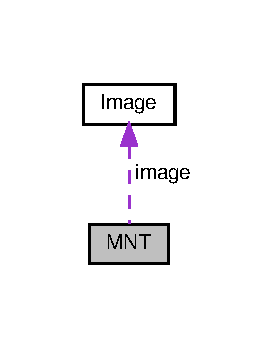
\includegraphics[width=132pt]{structMNT__coll__graph}
\end{center}
\end{figure}
\subsection*{Public Attributes}
\begin{DoxyCompactItemize}
\item 
\mbox{\Hypertarget{structMNT_a8626ef7ebc59484acd44ae4a3fab6fde}\label{structMNT_a8626ef7ebc59484acd44ae4a3fab6fde}} 
float {\bfseries xmin} = 0
\item 
\mbox{\Hypertarget{structMNT_aa1335893335ca42e17ce1859b8bb620f}\label{structMNT_aa1335893335ca42e17ce1859b8bb620f}} 
float {\bfseries xmax} = 0
\item 
\mbox{\Hypertarget{structMNT_ae6b46ea3a14d8ece99baf7b342165074}\label{structMNT_ae6b46ea3a14d8ece99baf7b342165074}} 
float {\bfseries ymin} = 0
\item 
\mbox{\Hypertarget{structMNT_a319e2c8bc5dbc576c5fc1450526aa459}\label{structMNT_a319e2c8bc5dbc576c5fc1450526aa459}} 
float {\bfseries ymax} = 0
\item 
\mbox{\Hypertarget{structMNT_a313da80d0a8fd24ba56ba51e070c29b2}\label{structMNT_a313da80d0a8fd24ba56ba51e070c29b2}} 
float {\bfseries min\+\_\+elevation} = 0
\item 
\mbox{\Hypertarget{structMNT_a0fa2bb2fc8258a96212568496d860bf1}\label{structMNT_a0fa2bb2fc8258a96212568496d860bf1}} 
float {\bfseries max\+\_\+elevation} = 0
\item 
\mbox{\Hypertarget{structMNT_ab5ae1542f4759c4b6514b852dfda969a}\label{structMNT_ab5ae1542f4759c4b6514b852dfda969a}} 
bool {\bfseries triangulation} = false
\item 
\mbox{\Hypertarget{structMNT_aad42a6c005fe6a63f7792cca148f898d}\label{structMNT_aad42a6c005fe6a63f7792cca148f898d}} 
std\+::map$<$ std\+::pair$<$ float, float $>$, float $>$ {\bfseries elevations}
\item 
\mbox{\Hypertarget{structMNT_a37602fb86c7aeb6b974a385d7c20bf48}\label{structMNT_a37602fb86c7aeb6b974a385d7c20bf48}} 
\hyperlink{classImage}{Image} {\bfseries image}
\end{DoxyCompactItemize}


\subsection{Detailed Description}
Digital Terrain Model structure (D\+TM or \hyperlink{structMNT}{M\+NT} in French) composed of\+: 


\begin{DoxyItemize}
\item Some parameters (xmin, xmax, ymin, yman, min\+\_\+elevation, max\+\_\+elevation, triangulation)
\item All the (x,y) coordinates of the sampled terrain and their corresponding elevation
\item An image representing the sampled terrain
\end{DoxyItemize}

Details about attributes\+: 
\begin{DoxyParams}{Parameters}
{\em xmin} & a constant float giving the minimal x coordinate on the sampled terrain \\
\hline
{\em xmax} & a constant float giving the maximal x coordinate on the sampled terrain \\
\hline
{\em ymin} & a constant float giving the minimal y coordinate on the sampled terrain \\
\hline
{\em ymax} & a constant float giving the maximal y coordinate on the sampled terrain \\
\hline
{\em triangulation} & a boolean indicating whether Delaunay\textquotesingle{}s is to be performed \\
\hline
{\em elevations} & a map of pair of floating coordinates (x,y) associated to the floating altitude of the point on the terrain \\
\hline
{\em image} & an \hyperlink{classImage}{Image} object representing the Digital Terrain Model (final output of the program) \\
\hline
\end{DoxyParams}


The documentation for this struct was generated from the following file\+:\begin{DoxyCompactItemize}
\item 
src/\hyperlink{utils_8h}{utils.\+h}\end{DoxyCompactItemize}

\hypertarget{classPixel}{}\section{Pixel Class Reference}
\label{classPixel}\index{Pixel@{Pixel}}


A class defining a custom pixel \+: R\+GB components with custom attributes \+:  




{\ttfamily \#include $<$Pixel.\+h$>$}

\subsection*{Public Member Functions}
\begin{DoxyCompactItemize}
\item 
\mbox{\Hypertarget{classPixel_a27ad99a2f705e635c42d242d530d4756}\label{classPixel_a27ad99a2f705e635c42d242d530d4756}} 
\hyperlink{classPixel_a27ad99a2f705e635c42d242d530d4756}{Pixel} ()
\begin{DoxyCompactList}\small\item\em Default constructor \+: construct a new \hyperlink{classPixel}{Pixel} object. \end{DoxyCompactList}\item 
\hyperlink{classPixel_a9ba4bf2d33c6d503e30059e61a43c045}{Pixel} (int R, int G, int B)
\begin{DoxyCompactList}\small\item\em Construct a new \hyperlink{classPixel}{Pixel} object. \end{DoxyCompactList}\item 
int \hyperlink{classPixel_ab2a26e47e90930b95012d56ca4dab3c0}{get\+\_\+R} () const
\begin{DoxyCompactList}\small\item\em Get the R component. \end{DoxyCompactList}\item 
int \hyperlink{classPixel_a7b8fb5740fe9ba2ff2960aa6d144cafe}{get\+\_\+G} () const
\begin{DoxyCompactList}\small\item\em Get the G component. \end{DoxyCompactList}\item 
int \hyperlink{classPixel_a50ea40ab4b069cd9cebe3a4d006466b4}{get\+\_\+B} () const
\begin{DoxyCompactList}\small\item\em Get the B component. \end{DoxyCompactList}\item 
float \hyperlink{classPixel_a07decaf3ba6ff526c8fa53fd730e9705}{get\+\_\+x} () const
\begin{DoxyCompactList}\small\item\em Get the x theoretical coordinate of the pixel on the terrain. \end{DoxyCompactList}\item 
float \hyperlink{classPixel_a6fcdc22470b74d9c1f704d0e670176ca}{get\+\_\+y} () const
\begin{DoxyCompactList}\small\item\em Get the y theoretical coordinate of the pixel on the terrain. \end{DoxyCompactList}\item 
const std\+::vector$<$ int $>$ $\ast$ \hyperlink{classPixel_a93366a506c032d97b25230469f0ca507}{get\+\_\+triangles\+\_\+indexes} () const
\begin{DoxyCompactList}\small\item\em Get the possible triangles\textquotesingle{} indexes for the pixel. Enable to identify to which triangular zone of the terrain the pixel belongs to. \end{DoxyCompactList}\item 
void \hyperlink{classPixel_a209745683886a3ccffd14e960edbed6c}{set\+\_\+\+R\+GB} (float elevation, const float min\+\_\+elevation, const float max\+\_\+elevation)
\begin{DoxyCompactList}\small\item\em Set the R\+GB components. \end{DoxyCompactList}\item 
void \hyperlink{classPixel_a51eafb0e5972c7f0f435354247a56966}{set\+\_\+gray\+\_\+intensity} (float elevation, const float min\+\_\+elevation, const float max\+\_\+elevation)
\begin{DoxyCompactList}\small\item\em Set the the R\+GB components for grayscale images. \end{DoxyCompactList}\item 
void \hyperlink{classPixel_af3245cdbe500abac1ff2af1575c5770f}{set\+\_\+x\+\_\+y} (int i, int j, const int img\+\_\+width, const int img\+\_\+height, const float xmin, const float xmax, const float ymin, const float ymax)
\begin{DoxyCompactList}\small\item\em Set the theoretical coordinates (x,y) of the pixel on the terrain (projection) \end{DoxyCompactList}\item 
void \hyperlink{classPixel_a9adc1965e90a981eb8723087b41a87cd}{add\+\_\+triangle\+\_\+index} (int index)
\begin{DoxyCompactList}\small\item\em Add the index of a possible triangular zone of belonging. \end{DoxyCompactList}\end{DoxyCompactItemize}


\subsection{Detailed Description}
A class defining a custom pixel \+: R\+GB components with custom attributes \+: 


\begin{DoxyItemize}
\item (x,y) theoretical coordinates in the terrain
\item the associated triangular zones after Delaunay\textquotesingle{}s triangulation of the terrain (if applicable) 
\end{DoxyItemize}

\subsection{Constructor \& Destructor Documentation}
\mbox{\Hypertarget{classPixel_a9ba4bf2d33c6d503e30059e61a43c045}\label{classPixel_a9ba4bf2d33c6d503e30059e61a43c045}} 
\index{Pixel@{Pixel}!Pixel@{Pixel}}
\index{Pixel@{Pixel}!Pixel@{Pixel}}
\subsubsection{\texorpdfstring{Pixel()}{Pixel()}}
{\footnotesize\ttfamily Pixel\+::\+Pixel (\begin{DoxyParamCaption}\item[{int}]{R,  }\item[{int}]{G,  }\item[{int}]{B }\end{DoxyParamCaption})}



Construct a new \hyperlink{classPixel}{Pixel} object. 


\begin{DoxyParams}{Parameters}
{\em R} & an integer \+: the red component of the pixel \\
\hline
{\em G} & an integer \+: the green component of the pixel \\
\hline
{\em B} & an integer \+: the blue component of the pixel \\
\hline
\end{DoxyParams}


\subsection{Member Function Documentation}
\mbox{\Hypertarget{classPixel_a9adc1965e90a981eb8723087b41a87cd}\label{classPixel_a9adc1965e90a981eb8723087b41a87cd}} 
\index{Pixel@{Pixel}!add\+\_\+triangle\+\_\+index@{add\+\_\+triangle\+\_\+index}}
\index{add\+\_\+triangle\+\_\+index@{add\+\_\+triangle\+\_\+index}!Pixel@{Pixel}}
\subsubsection{\texorpdfstring{add\+\_\+triangle\+\_\+index()}{add\_triangle\_index()}}
{\footnotesize\ttfamily void Pixel\+::add\+\_\+triangle\+\_\+index (\begin{DoxyParamCaption}\item[{int}]{index }\end{DoxyParamCaption})}



Add the index of a possible triangular zone of belonging. 


\begin{DoxyParams}{Parameters}
{\em index} & an integer giving the index of the triangle in Delaunay\textquotesingle{}s vector \\
\hline
\end{DoxyParams}
\mbox{\Hypertarget{classPixel_a50ea40ab4b069cd9cebe3a4d006466b4}\label{classPixel_a50ea40ab4b069cd9cebe3a4d006466b4}} 
\index{Pixel@{Pixel}!get\+\_\+B@{get\+\_\+B}}
\index{get\+\_\+B@{get\+\_\+B}!Pixel@{Pixel}}
\subsubsection{\texorpdfstring{get\+\_\+\+B()}{get\_B()}}
{\footnotesize\ttfamily int Pixel\+::get\+\_\+B (\begin{DoxyParamCaption}{ }\end{DoxyParamCaption}) const}



Get the B component. 

\begin{DoxyReturn}{Returns}
int 
\end{DoxyReturn}
\mbox{\Hypertarget{classPixel_a7b8fb5740fe9ba2ff2960aa6d144cafe}\label{classPixel_a7b8fb5740fe9ba2ff2960aa6d144cafe}} 
\index{Pixel@{Pixel}!get\+\_\+G@{get\+\_\+G}}
\index{get\+\_\+G@{get\+\_\+G}!Pixel@{Pixel}}
\subsubsection{\texorpdfstring{get\+\_\+\+G()}{get\_G()}}
{\footnotesize\ttfamily int Pixel\+::get\+\_\+G (\begin{DoxyParamCaption}{ }\end{DoxyParamCaption}) const}



Get the G component. 

\begin{DoxyReturn}{Returns}
int 
\end{DoxyReturn}
\mbox{\Hypertarget{classPixel_ab2a26e47e90930b95012d56ca4dab3c0}\label{classPixel_ab2a26e47e90930b95012d56ca4dab3c0}} 
\index{Pixel@{Pixel}!get\+\_\+R@{get\+\_\+R}}
\index{get\+\_\+R@{get\+\_\+R}!Pixel@{Pixel}}
\subsubsection{\texorpdfstring{get\+\_\+\+R()}{get\_R()}}
{\footnotesize\ttfamily int Pixel\+::get\+\_\+R (\begin{DoxyParamCaption}{ }\end{DoxyParamCaption}) const}



Get the R component. 

\begin{DoxyReturn}{Returns}
int 
\end{DoxyReturn}
\mbox{\Hypertarget{classPixel_a93366a506c032d97b25230469f0ca507}\label{classPixel_a93366a506c032d97b25230469f0ca507}} 
\index{Pixel@{Pixel}!get\+\_\+triangles\+\_\+indexes@{get\+\_\+triangles\+\_\+indexes}}
\index{get\+\_\+triangles\+\_\+indexes@{get\+\_\+triangles\+\_\+indexes}!Pixel@{Pixel}}
\subsubsection{\texorpdfstring{get\+\_\+triangles\+\_\+indexes()}{get\_triangles\_indexes()}}
{\footnotesize\ttfamily const vector$<$ int $>$ $\ast$ Pixel\+::get\+\_\+triangles\+\_\+indexes (\begin{DoxyParamCaption}{ }\end{DoxyParamCaption}) const}



Get the possible triangles\textquotesingle{} indexes for the pixel. Enable to identify to which triangular zone of the terrain the pixel belongs to. 

\begin{DoxyReturn}{Returns}
const std\+::vector$<$int$>$$\ast$ a pointer to the vector of indexes 
\end{DoxyReturn}
\mbox{\Hypertarget{classPixel_a07decaf3ba6ff526c8fa53fd730e9705}\label{classPixel_a07decaf3ba6ff526c8fa53fd730e9705}} 
\index{Pixel@{Pixel}!get\+\_\+x@{get\+\_\+x}}
\index{get\+\_\+x@{get\+\_\+x}!Pixel@{Pixel}}
\subsubsection{\texorpdfstring{get\+\_\+x()}{get\_x()}}
{\footnotesize\ttfamily float Pixel\+::get\+\_\+x (\begin{DoxyParamCaption}{ }\end{DoxyParamCaption}) const}



Get the x theoretical coordinate of the pixel on the terrain. 

\begin{DoxyReturn}{Returns}
float 
\end{DoxyReturn}
\mbox{\Hypertarget{classPixel_a6fcdc22470b74d9c1f704d0e670176ca}\label{classPixel_a6fcdc22470b74d9c1f704d0e670176ca}} 
\index{Pixel@{Pixel}!get\+\_\+y@{get\+\_\+y}}
\index{get\+\_\+y@{get\+\_\+y}!Pixel@{Pixel}}
\subsubsection{\texorpdfstring{get\+\_\+y()}{get\_y()}}
{\footnotesize\ttfamily float Pixel\+::get\+\_\+y (\begin{DoxyParamCaption}{ }\end{DoxyParamCaption}) const}



Get the y theoretical coordinate of the pixel on the terrain. 

\begin{DoxyReturn}{Returns}
float 
\end{DoxyReturn}
\mbox{\Hypertarget{classPixel_a51eafb0e5972c7f0f435354247a56966}\label{classPixel_a51eafb0e5972c7f0f435354247a56966}} 
\index{Pixel@{Pixel}!set\+\_\+gray\+\_\+intensity@{set\+\_\+gray\+\_\+intensity}}
\index{set\+\_\+gray\+\_\+intensity@{set\+\_\+gray\+\_\+intensity}!Pixel@{Pixel}}
\subsubsection{\texorpdfstring{set\+\_\+gray\+\_\+intensity()}{set\_gray\_intensity()}}
{\footnotesize\ttfamily void Pixel\+::set\+\_\+gray\+\_\+intensity (\begin{DoxyParamCaption}\item[{float}]{elevation,  }\item[{const float}]{min\+\_\+elevation,  }\item[{const float}]{max\+\_\+elevation }\end{DoxyParamCaption})}



Set the the R\+GB components for grayscale images. 


\begin{DoxyParams}{Parameters}
{\em elevation} & a float giving the altitude of the corresponding point on the terrain \\
\hline
{\em min\+\_\+elevation} & a float giving the minimal altitude on the terrain \\
\hline
{\em max\+\_\+elevation} & a float giving the maximal altitude on the terrain \\
\hline
\end{DoxyParams}
\mbox{\Hypertarget{classPixel_a209745683886a3ccffd14e960edbed6c}\label{classPixel_a209745683886a3ccffd14e960edbed6c}} 
\index{Pixel@{Pixel}!set\+\_\+\+R\+GB@{set\+\_\+\+R\+GB}}
\index{set\+\_\+\+R\+GB@{set\+\_\+\+R\+GB}!Pixel@{Pixel}}
\subsubsection{\texorpdfstring{set\+\_\+\+R\+G\+B()}{set\_RGB()}}
{\footnotesize\ttfamily void Pixel\+::set\+\_\+\+R\+GB (\begin{DoxyParamCaption}\item[{float}]{elevation,  }\item[{const float}]{min\+\_\+elevation,  }\item[{const float}]{max\+\_\+elevation }\end{DoxyParamCaption})}



Set the R\+GB components. 


\begin{DoxyParams}{Parameters}
{\em elevation} & a float giving the altitude of the corresponding point on the terrain \\
\hline
{\em min\+\_\+elevation} & a float giving the minimal altitude on the terrain \\
\hline
{\em max\+\_\+elevation} & a float giving the maximal altitude on the terrain \\
\hline
\end{DoxyParams}
Create a simple rainbow colormap. To convert a scalar to a rainbow, we divide the scalar into four groups. Then based on which group we are in, we perform one of the following linear interpolations\+:


\begin{DoxyItemize}
\item Group 1\+: Red is maximum (255), blue is zero, and green varies linearly from 0 to 255.
\item Group 2\+: Green is kept maximum and blue is still zero. Red varies linearly from 255 to 0.
\item Group 3\+: Keep red at zero and green and maximum. Blue varies linearly from 0 to 255.
\item Group 4\+: Red is kept at zero and blue at maximum. Green varies linearly from 255 to 0.
\end{DoxyItemize}

This ordering follows the image in the Wikipedia article. One downside of this approach is that it will vary from red to blue as f varies from 0 to 1. Typically, we want the opposite, with 0 mapping to blue and 1 to red. So we simply invert the scalar as a=1-\/f. \mbox{\Hypertarget{classPixel_af3245cdbe500abac1ff2af1575c5770f}\label{classPixel_af3245cdbe500abac1ff2af1575c5770f}} 
\index{Pixel@{Pixel}!set\+\_\+x\+\_\+y@{set\+\_\+x\+\_\+y}}
\index{set\+\_\+x\+\_\+y@{set\+\_\+x\+\_\+y}!Pixel@{Pixel}}
\subsubsection{\texorpdfstring{set\+\_\+x\+\_\+y()}{set\_x\_y()}}
{\footnotesize\ttfamily void Pixel\+::set\+\_\+x\+\_\+y (\begin{DoxyParamCaption}\item[{int}]{i,  }\item[{int}]{j,  }\item[{const int}]{img\+\_\+width,  }\item[{const int}]{img\+\_\+height,  }\item[{const float}]{xmin,  }\item[{const float}]{xmax,  }\item[{const float}]{ymin,  }\item[{const float}]{ymax }\end{DoxyParamCaption})}



Set the theoretical coordinates (x,y) of the pixel on the terrain (projection) 


\begin{DoxyParams}{Parameters}
{\em i} & an integer giving the line of the pixel \\
\hline
{\em j} & an interger giving the column of the pixel \\
\hline
{\em img\+\_\+width} & a constant integer \\
\hline
{\em img\+\_\+height} & a constant integer \\
\hline
{\em xmin} & a constant float giving the minimal x coordinate on the sampled terrain \\
\hline
{\em xmax} & a constant float giving the maximal x coordinate on the sampled terrain \\
\hline
{\em ymin} & a constant float giving the minimal y coordinate on the sampled terrain \\
\hline
{\em ymax} & a constant float giving the maximal y coordinate on the sampled terrain \\
\hline
\end{DoxyParams}


The documentation for this class was generated from the following files\+:\begin{DoxyCompactItemize}
\item 
src/\hyperlink{Pixel_8h}{Pixel.\+h}\item 
src/Pixel.\+cpp\end{DoxyCompactItemize}

\chapter{File Documentation}
\hypertarget{delaunator_8hpp}{}\section{src/delaunator.hpp File Reference}
\label{delaunator_8hpp}\index{src/delaunator.\+hpp@{src/delaunator.\+hpp}}
{\ttfamily \#include $<$algorithm$>$}\newline
{\ttfamily \#include $<$cmath$>$}\newline
{\ttfamily \#include $<$exception$>$}\newline
{\ttfamily \#include $<$iostream$>$}\newline
{\ttfamily \#include $<$limits$>$}\newline
{\ttfamily \#include $<$memory$>$}\newline
{\ttfamily \#include $<$utility$>$}\newline
{\ttfamily \#include $<$vector$>$}\newline
Include dependency graph for delaunator.\+hpp\+:\nopagebreak
\begin{figure}[H]
\begin{center}
\leavevmode
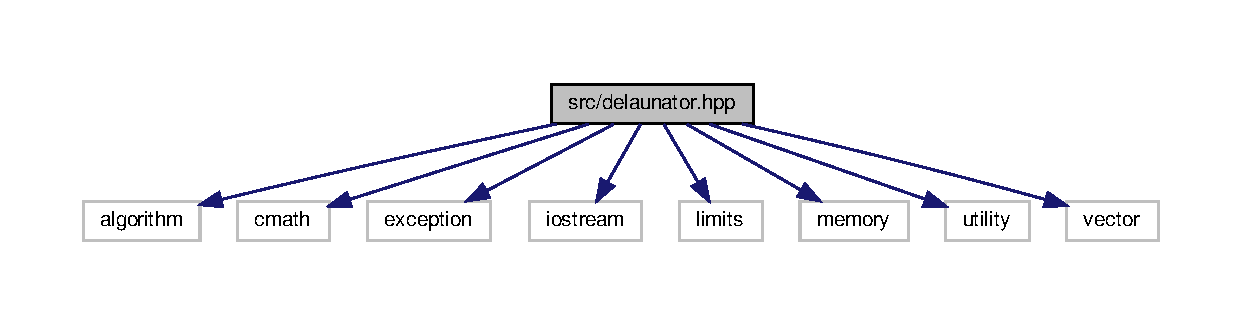
\includegraphics[width=350pt]{delaunator_8hpp__incl}
\end{center}
\end{figure}
\subsection*{Classes}
\begin{DoxyCompactItemize}
\item 
struct \hyperlink{structdelaunator_1_1compare}{delaunator\+::compare}
\item 
struct \hyperlink{structdelaunator_1_1DelaunatorPoint}{delaunator\+::\+Delaunator\+Point}
\item 
class \hyperlink{classdelaunator_1_1Delaunator}{delaunator\+::\+Delaunator}
\end{DoxyCompactItemize}
\subsection*{Functions}
\begin{DoxyCompactItemize}
\item 
\mbox{\Hypertarget{delaunator_8hpp_a3bf510ee4922ac9e97b969e0c405e98b}\label{delaunator_8hpp_a3bf510ee4922ac9e97b969e0c405e98b}} 
size\+\_\+t {\bfseries delaunator\+::fast\+\_\+mod} (const size\+\_\+t i, const size\+\_\+t c)
\item 
\mbox{\Hypertarget{delaunator_8hpp_aa0fda089647a091b92b8548ad3c0f100}\label{delaunator_8hpp_aa0fda089647a091b92b8548ad3c0f100}} 
double {\bfseries delaunator\+::sum} (const std\+::vector$<$ double $>$ \&x)
\item 
\mbox{\Hypertarget{delaunator_8hpp_a9e2a3ffc907659930fa0edad646d49dc}\label{delaunator_8hpp_a9e2a3ffc907659930fa0edad646d49dc}} 
double {\bfseries delaunator\+::dist} (const double ax, const double ay, const double bx, const double by)
\item 
\mbox{\Hypertarget{delaunator_8hpp_a41cf84f19316cc7fb922b160b35af8f9}\label{delaunator_8hpp_a41cf84f19316cc7fb922b160b35af8f9}} 
double {\bfseries delaunator\+::circumradius} (const double ax, const double ay, const double bx, const double by, const double cx, const double cy)
\item 
\mbox{\Hypertarget{delaunator_8hpp_aebc9337156dd42cb19372d15119525db}\label{delaunator_8hpp_aebc9337156dd42cb19372d15119525db}} 
bool {\bfseries delaunator\+::orient} (const double px, const double py, const double qx, const double qy, const double rx, const double ry)
\item 
\mbox{\Hypertarget{delaunator_8hpp_a4130131df38cca8830863a2209794347}\label{delaunator_8hpp_a4130131df38cca8830863a2209794347}} 
std\+::pair$<$ double, double $>$ {\bfseries delaunator\+::circumcenter} (const double ax, const double ay, const double bx, const double by, const double cx, const double cy)
\item 
\mbox{\Hypertarget{delaunator_8hpp_a5e7a51e33a9d4eea7ac9ca2e38aa7fa6}\label{delaunator_8hpp_a5e7a51e33a9d4eea7ac9ca2e38aa7fa6}} 
bool {\bfseries delaunator\+::in\+\_\+circle} (const double ax, const double ay, const double bx, const double by, const double cx, const double cy, const double px, const double py)
\item 
\mbox{\Hypertarget{delaunator_8hpp_acd98fbc5da3dc94d8ee30d704eed18e9}\label{delaunator_8hpp_acd98fbc5da3dc94d8ee30d704eed18e9}} 
bool {\bfseries delaunator\+::check\+\_\+pts\+\_\+equal} (double x1, double y1, double x2, double y2)
\item 
\mbox{\Hypertarget{delaunator_8hpp_a3cdb1c51389d918a83f3db7264891305}\label{delaunator_8hpp_a3cdb1c51389d918a83f3db7264891305}} 
double {\bfseries delaunator\+::pseudo\+\_\+angle} (const double dx, const double dy)
\end{DoxyCompactItemize}
\subsection*{Variables}
\begin{DoxyCompactItemize}
\item 
\mbox{\Hypertarget{delaunator_8hpp_a2bba00df8f04d31916772f7ebc15734c}\label{delaunator_8hpp_a2bba00df8f04d31916772f7ebc15734c}} 
constexpr double {\bfseries delaunator\+::\+E\+P\+S\+I\+L\+ON} = std\+::numeric\+\_\+limits$<$double$>$\+::epsilon()
\item 
\mbox{\Hypertarget{delaunator_8hpp_acb0d4406320caf27239204ed6e5809bf}\label{delaunator_8hpp_acb0d4406320caf27239204ed6e5809bf}} 
constexpr std\+::size\+\_\+t {\bfseries delaunator\+::\+I\+N\+V\+A\+L\+I\+D\+\_\+\+I\+N\+D\+EX} = std\+::numeric\+\_\+limits$<$std\+::size\+\_\+t$>$\+::max()
\end{DoxyCompactItemize}

\hypertarget{Image_8h}{}\section{src/\+Image.h File Reference}
\label{Image_8h}\index{src/\+Image.\+h@{src/\+Image.\+h}}
{\ttfamily \#include $<$cstdlib$>$}\newline
{\ttfamily \#include $<$map$>$}\newline
{\ttfamily \#include \char`\"{}Pixel.\+h\char`\"{}}\newline
Include dependency graph for Image.\+h\+:\nopagebreak
\begin{figure}[H]
\begin{center}
\leavevmode
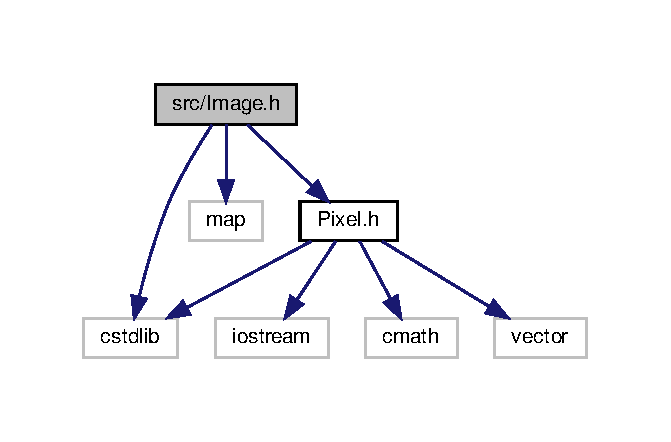
\includegraphics[width=322pt]{Image_8h__incl}
\end{center}
\end{figure}
This graph shows which files directly or indirectly include this file\+:\nopagebreak
\begin{figure}[H]
\begin{center}
\leavevmode
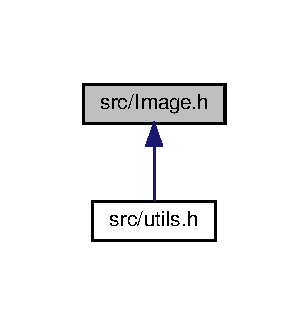
\includegraphics[width=148pt]{Image_8h__dep__incl}
\end{center}
\end{figure}
\subsection*{Classes}
\begin{DoxyCompactItemize}
\item 
class \hyperlink{classImage}{Image}
\begin{DoxyCompactList}\small\item\em A class defining a custom image with some classic attributes \+: \end{DoxyCompactList}\end{DoxyCompactItemize}

\hypertarget{Pixel_8h}{}\section{src/\+Pixel.h File Reference}
\label{Pixel_8h}\index{src/\+Pixel.\+h@{src/\+Pixel.\+h}}
{\ttfamily \#include $<$cstdlib$>$}\newline
{\ttfamily \#include $<$iostream$>$}\newline
{\ttfamily \#include $<$cmath$>$}\newline
{\ttfamily \#include $<$vector$>$}\newline
Include dependency graph for Pixel.\+h\+:\nopagebreak
\begin{figure}[H]
\begin{center}
\leavevmode
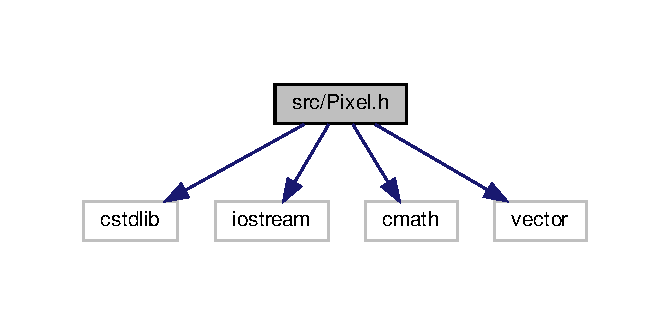
\includegraphics[width=322pt]{Pixel_8h__incl}
\end{center}
\end{figure}
This graph shows which files directly or indirectly include this file\+:\nopagebreak
\begin{figure}[H]
\begin{center}
\leavevmode
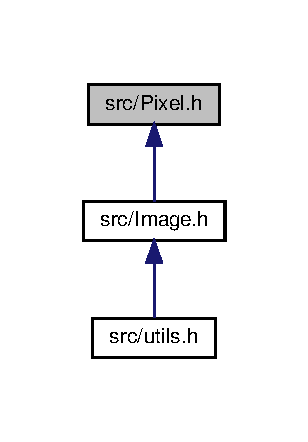
\includegraphics[width=148pt]{Pixel_8h__dep__incl}
\end{center}
\end{figure}
\subsection*{Classes}
\begin{DoxyCompactItemize}
\item 
class \hyperlink{classPixel}{Pixel}
\begin{DoxyCompactList}\small\item\em A class defining a custom pixel \+: R\+GB components with custom attributes \+: \end{DoxyCompactList}\end{DoxyCompactItemize}

\hypertarget{utils_8h}{}\section{src/utils.h File Reference}
\label{utils_8h}\index{src/utils.\+h@{src/utils.\+h}}


A file containing useful structure and functions to generate a D\+TM or \hyperlink{structMNT}{M\+NT} in French.  


{\ttfamily \#include $<$cstdlib$>$}\newline
{\ttfamily \#include $<$iostream$>$}\newline
{\ttfamily \#include $<$fstream$>$}\newline
{\ttfamily \#include $<$string$>$}\newline
{\ttfamily \#include $<$proj.\+h$>$}\newline
{\ttfamily \#include $<$cstdio$>$}\newline
{\ttfamily \#include $<$vector$>$}\newline
{\ttfamily \#include $<$map$>$}\newline
{\ttfamily \#include \char`\"{}Image.\+h\char`\"{}}\newline
Include dependency graph for utils.\+h\+:\nopagebreak
\begin{figure}[H]
\begin{center}
\leavevmode
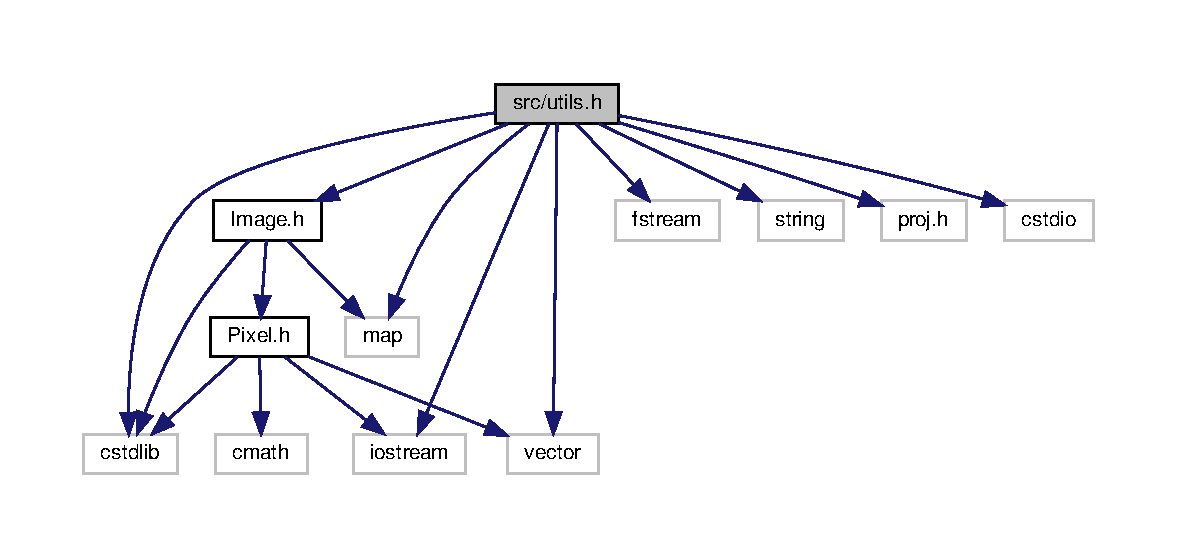
\includegraphics[width=350pt]{utils_8h__incl}
\end{center}
\end{figure}
\subsection*{Classes}
\begin{DoxyCompactItemize}
\item 
struct \hyperlink{structMNT}{M\+NT}
\begin{DoxyCompactList}\small\item\em Digital Terrain Model structure (D\+TM or \hyperlink{structMNT}{M\+NT} in French) composed of\+: \end{DoxyCompactList}\end{DoxyCompactItemize}
\subsection*{Functions}
\begin{DoxyCompactItemize}
\item 
\hyperlink{structMNT}{M\+NT} \hyperlink{utils_8h_af26108b5c5ba4562d8cc73e2cde8b994}{read\+\_\+data} (const char $\ast$file\+\_\+path, std\+::vector$<$ double $>$ \&coords, const int image\+\_\+width, bool triangulation, bool is\+\_\+gray, bool is\+\_\+binary)
\begin{DoxyCompactList}\small\item\em Read the raw sampled data of the terrain and init an \hyperlink{structMNT}{M\+NT} object. The raw data have 3 coordinates (longitude, latitude, elevation) to be projected -\/ thanks to Lambert 93 projection -\/ into (northing, easting, elevation). They are saved into {\bfseries coords} vector and an \hyperlink{structMNT}{M\+NT} object is created. \end{DoxyCompactList}\item 
void \hyperlink{utils_8h_a2398d95aa1a7f7483e5b74e06f57c85a}{write\+\_\+image} (const \hyperlink{classImage}{Image} \&image, std\+::string file\+\_\+name)
\begin{DoxyCompactList}\small\item\em Write an image file according to its encoding parameters. \end{DoxyCompactList}\item 
void \hyperlink{utils_8h_a02e38d3b2d8f2d521e4b5747d397aefd}{convert\+\_\+data\+\_\+to\+\_\+pixels} (\hyperlink{structMNT}{M\+NT} \&raster)
\begin{DoxyCompactList}\small\item\em Convert raw data elevations into R\+GB components for the image\textquotesingle{}s pixels. \end{DoxyCompactList}\item 
void \hyperlink{utils_8h_a3fe45b5304a807b6b17248f452106bd9}{convert\+\_\+data\+\_\+to\+\_\+pixels\+\_\+delaunay} (std\+::vector$<$ double $>$ \&coords, \hyperlink{structMNT}{M\+NT} \&raster)
\begin{DoxyCompactList}\small\item\em Convert raw data elevations into R\+GB components for the image\textquotesingle{}s pixels after performing Delaunay\textquotesingle{}s triangulation of the points of the terrain. \end{DoxyCompactList}\item 
void \hyperlink{utils_8h_a26d8307e7a6d814f560b3e2aba762850}{associate\+\_\+triangle\+\_\+summits\+\_\+to\+\_\+pixels} (\hyperlink{structMNT}{M\+NT} \&raster, const std\+::vector$<$ size\+\_\+t $>$ \&triangles, const std\+::vector$<$ double $>$ \&coords)
\begin{DoxyCompactList}\small\item\em Only applicable if Delaunay\textquotesingle{}s triangulation is performed on the sampled points of the terrain. Associate the possible triangular zones of belonging for each pixel of the image. \end{DoxyCompactList}\end{DoxyCompactItemize}


\subsection{Detailed Description}
A file containing useful structure and functions to generate a D\+TM or \hyperlink{structMNT}{M\+NT} in French. 



\subsection{Function Documentation}
\mbox{\Hypertarget{utils_8h_a26d8307e7a6d814f560b3e2aba762850}\label{utils_8h_a26d8307e7a6d814f560b3e2aba762850}} 
\index{utils.\+h@{utils.\+h}!associate\+\_\+triangle\+\_\+summits\+\_\+to\+\_\+pixels@{associate\+\_\+triangle\+\_\+summits\+\_\+to\+\_\+pixels}}
\index{associate\+\_\+triangle\+\_\+summits\+\_\+to\+\_\+pixels@{associate\+\_\+triangle\+\_\+summits\+\_\+to\+\_\+pixels}!utils.\+h@{utils.\+h}}
\subsubsection{\texorpdfstring{associate\+\_\+triangle\+\_\+summits\+\_\+to\+\_\+pixels()}{associate\_triangle\_summits\_to\_pixels()}}
{\footnotesize\ttfamily void associate\+\_\+triangle\+\_\+summits\+\_\+to\+\_\+pixels (\begin{DoxyParamCaption}\item[{\hyperlink{structMNT}{M\+NT} \&}]{raster,  }\item[{const std\+::vector$<$ size\+\_\+t $>$ \&}]{triangles,  }\item[{const std\+::vector$<$ double $>$ \&}]{coords }\end{DoxyParamCaption})}



Only applicable if Delaunay\textquotesingle{}s triangulation is performed on the sampled points of the terrain. Associate the possible triangular zones of belonging for each pixel of the image. 


\begin{DoxyParams}{Parameters}
{\em raster} & an \hyperlink{structMNT}{M\+NT} object \\
\hline
{\em triangles} & a vector containing all the summits of the triangles determined by Delaunay\textquotesingle{}s triangulation of the terrain. \\
\hline
{\em coords} & a vector of the coordinates (x,y) of the sampled data of the terrain \\
\hline
\end{DoxyParams}
\mbox{\Hypertarget{utils_8h_a02e38d3b2d8f2d521e4b5747d397aefd}\label{utils_8h_a02e38d3b2d8f2d521e4b5747d397aefd}} 
\index{utils.\+h@{utils.\+h}!convert\+\_\+data\+\_\+to\+\_\+pixels@{convert\+\_\+data\+\_\+to\+\_\+pixels}}
\index{convert\+\_\+data\+\_\+to\+\_\+pixels@{convert\+\_\+data\+\_\+to\+\_\+pixels}!utils.\+h@{utils.\+h}}
\subsubsection{\texorpdfstring{convert\+\_\+data\+\_\+to\+\_\+pixels()}{convert\_data\_to\_pixels()}}
{\footnotesize\ttfamily void convert\+\_\+data\+\_\+to\+\_\+pixels (\begin{DoxyParamCaption}\item[{\hyperlink{structMNT}{M\+NT} \&}]{raster }\end{DoxyParamCaption})}



Convert raw data elevations into R\+GB components for the image\textquotesingle{}s pixels. 


\begin{DoxyParams}{Parameters}
{\em raster} & an \hyperlink{structMNT}{M\+NT} object \\
\hline
\end{DoxyParams}
\mbox{\Hypertarget{utils_8h_a3fe45b5304a807b6b17248f452106bd9}\label{utils_8h_a3fe45b5304a807b6b17248f452106bd9}} 
\index{utils.\+h@{utils.\+h}!convert\+\_\+data\+\_\+to\+\_\+pixels\+\_\+delaunay@{convert\+\_\+data\+\_\+to\+\_\+pixels\+\_\+delaunay}}
\index{convert\+\_\+data\+\_\+to\+\_\+pixels\+\_\+delaunay@{convert\+\_\+data\+\_\+to\+\_\+pixels\+\_\+delaunay}!utils.\+h@{utils.\+h}}
\subsubsection{\texorpdfstring{convert\+\_\+data\+\_\+to\+\_\+pixels\+\_\+delaunay()}{convert\_data\_to\_pixels\_delaunay()}}
{\footnotesize\ttfamily void convert\+\_\+data\+\_\+to\+\_\+pixels\+\_\+delaunay (\begin{DoxyParamCaption}\item[{std\+::vector$<$ double $>$ \&}]{coords,  }\item[{\hyperlink{structMNT}{M\+NT} \&}]{raster }\end{DoxyParamCaption})}



Convert raw data elevations into R\+GB components for the image\textquotesingle{}s pixels after performing Delaunay\textquotesingle{}s triangulation of the points of the terrain. 


\begin{DoxyParams}{Parameters}
{\em coords} & a vector of the coordinates (x,y) of the sampled data of the terrain \\
\hline
{\em raster} & an \hyperlink{structMNT}{M\+NT} object \\
\hline
\end{DoxyParams}
\mbox{\Hypertarget{utils_8h_af26108b5c5ba4562d8cc73e2cde8b994}\label{utils_8h_af26108b5c5ba4562d8cc73e2cde8b994}} 
\index{utils.\+h@{utils.\+h}!read\+\_\+data@{read\+\_\+data}}
\index{read\+\_\+data@{read\+\_\+data}!utils.\+h@{utils.\+h}}
\subsubsection{\texorpdfstring{read\+\_\+data()}{read\_data()}}
{\footnotesize\ttfamily \hyperlink{structMNT}{M\+NT} read\+\_\+data (\begin{DoxyParamCaption}\item[{const char $\ast$}]{file\+\_\+path,  }\item[{std\+::vector$<$ double $>$ \&}]{coords,  }\item[{const int}]{image\+\_\+width,  }\item[{bool}]{triangulation,  }\item[{bool}]{is\+\_\+gray,  }\item[{bool}]{is\+\_\+binary }\end{DoxyParamCaption})}



Read the raw sampled data of the terrain and init an \hyperlink{structMNT}{M\+NT} object. The raw data have 3 coordinates (longitude, latitude, elevation) to be projected -\/ thanks to Lambert 93 projection -\/ into (northing, easting, elevation). They are saved into {\bfseries coords} vector and an \hyperlink{structMNT}{M\+NT} object is created. 


\begin{DoxyParams}{Parameters}
{\em file\+\_\+path} & a string indicating the full-\/path or relative one to the text document containing the terrain data to read \\
\hline
{\em coords} & a vector of the coordinates (x,y) of the sampled data of the terrain \\
\hline
{\em image\+\_\+width} & an integer chosen by the user to define the resolution if the image output \\
\hline
{\em triangulation} & a bool to indicate whether Delaunay\textquotesingle{}s triangulation is to be performed on the (x,y) sampled coordinates of the terrain \\
\hline
{\em is\+\_\+gray} & a bool indicating if the output image should be in grayscale or in color \\
\hline
{\em is\+\_\+binary} & a bool indicating if the output image should be encoded in binary or not \\
\hline
\end{DoxyParams}
\begin{DoxyReturn}{Returns}
\hyperlink{structMNT}{M\+NT} object 
\end{DoxyReturn}
\mbox{\Hypertarget{utils_8h_a2398d95aa1a7f7483e5b74e06f57c85a}\label{utils_8h_a2398d95aa1a7f7483e5b74e06f57c85a}} 
\index{utils.\+h@{utils.\+h}!write\+\_\+image@{write\+\_\+image}}
\index{write\+\_\+image@{write\+\_\+image}!utils.\+h@{utils.\+h}}
\subsubsection{\texorpdfstring{write\+\_\+image()}{write\_image()}}
{\footnotesize\ttfamily void write\+\_\+image (\begin{DoxyParamCaption}\item[{const \hyperlink{classImage}{Image} \&}]{image,  }\item[{std\+::string}]{file\+\_\+name }\end{DoxyParamCaption})}



Write an image file according to its encoding parameters. 


\begin{DoxyParams}{Parameters}
{\em image} & an \hyperlink{classImage}{Image} object \\
\hline
{\em file\+\_\+name} & a string giving the full path or relative one of the image file and the name of it. The file extension is determined thanks to the encoding parameters of the \hyperlink{classImage}{Image} object. \\
\hline
\end{DoxyParams}

%--- End generated contents ---

% Index
\backmatter
\newpage
\phantomsection
\clearemptydoublepage
\addcontentsline{toc}{chapter}{Index}
\printindex

\end{document}
